\documentclass[12pt]{article}
\usepackage[T2A]{fontenc}
\usepackage[utf8]{inputenc}
\usepackage{multirow}
\usepackage{caption}
\usepackage{subcaption}
\usepackage{amsmath}
\usepackage{amssymb}
\usepackage{changepage}
\usepackage{graphicx}
\usepackage{float}
\usepackage[english,russian]{babel}
\usepackage{amsmath, amsfonts, amssymb, amsthm, mathtools}
\usepackage{xcolor}
\usepackage{array}
\usepackage{hyperref}
\usepackage{physics}
\usepackage[top = 1.5cm, left = 1.5 cm, right = 1.5 cm, bottom = 3 cm]{geometry}
\usepackage{import}
\usepackage{xifthen}
\usepackage{pdfpages}
\usepackage{transparent}

\newcommand{\incfig}[1]{
    \import{./figures/}{#1.pdf_tex}
}

\title{Практика 1.}
\author{Шахматов Андрей, Б02-304}
\date{\today}

\begin{document}
\maketitle
\tableofcontents

\section{1.1}
$$M = \mathbb{Q} \times \{\frac{1}{n} \mid n \in \mathbb{N}\}$$
Внутренность $M$ - пустое множество, так как для любой $m = \left(\frac{p}{q}, \frac{1}{n}\right)$ 
и любой её окрестности $U$ есть точка $q = \left(i \in \mathbb{I}, \frac{1}{n}\right)$.
Граничными точками являются все прямые вида $y = \frac{1}{n} \mid n \in \mathbb{N}$ и $y = 0$.
Внешними точками является множество $ext M = \mathbb{R}^2 \setminus \partial M \setminus int M = \mathbb{R}^2 \setminus \{(x, y) \in \mathbb{R}^2 \mid y = 0 \land y = \frac{1}{n} \, n \in \mathbb{N}\}$.
Изолированных точек нет, так как $\forall m \in M$ и для любой её окрестности есть точка множества лежащая в этой окрестности.
Предельные точки совпадают с границей. 

\section{1.2}
$$f(x, y) = \frac{1}{\sqrt{xy}}$$
Множество определения $D_f = {(x, y) \in \mathbb{R}^2 \mid (x > 0 \land y > 0) \lor (x < 0 \land y < 0)}$
\begin{figure}[H]
    \centering
    \def\svgwidth{0.5\columnwidth}
    \incfig{P12}
    \caption{Область определения функции}
    \label{fig:P12}
\end{figure}
(a) $D_f$ - открыто, так как совпадает со своей внутреннстью. 
$D_f \cup {0}$ - не открыто, так как 0 - граничная точка. \\
(б) $D_f$ - не замкнуто
$D_f \cup {0}$ - не замкнуто, так как все точки на прямых $x =
0$ и $y = 0$ являются граничными и не лежат в множестве. \\
(в) Ни одно множество не компакт так как не замкнуто. \\
(г) $D_f$ - не связно, так как не линейно связно и открыто и находится в $\mathbb{R}^2$.
$D_f \cup {0}$ - связно, так как линейно связно. \\
(д) $D_f$ - не линейно связное, так как любая кривая должна проходить через $(0, 0) \not \in M$.
$D_f \cup {0}$ - линейно свзяно. \\
(е) $D_f$ - не область так как не связно.
$D_f \cup {0}$ - не область так как не открыто. \\
\section{1.3}
$$f(x, y) = \frac{x^3 + y^3}{x^2 + y^2}$$
Перейдём к замене $x = \rho\cos{\phi}$, $y = \rho\sin{\phi}$.
$$
|f(x, y)| = \rho |\frac{\sin^3{\phi} + \cos^3{\phi}}{\sin^2{\phi} + \cos^2{\phi}}| = \rho |\sin^3{\phi} + \cos^3{\phi}| \leq 2\rho
$$
Тогда при $x \to 0$ и $y \to 0$ выполняется $\rho \to 0 \Rightarrow |f(x, y)| \to 0 \Rightarrow f(x, y) \to 0$. 

\section{1.4}
(a) $$f(x, y) = \frac{x^3}{x^2 + y^2}$$
$$\lim_{x \to 0}{\lim_{y \to 0}{\frac{x^3}{x^2 + y^2}}} = \lim_{x \to 0}{x} = 0$$
$$\lim_{y \to 0}{\lim_{x \to 0}{\frac{x^3}{x^2 + y^2}}} = \lim_{y \to 0}{0} = 0$$
Введя замену $x = \rho\cos{\phi}$, $y = \rho\sin{\phi}$ получим 
$$|f(x, y)| = \rho |\cos^3{\phi}| \leq \rho \Rightarrow |f(x, y)| \to 0, \, \textrm{при} \, \rho \to 0$$ \\
(б) $$f(x, y) = \frac{x - y}{x + y}$$
$$\lim_{x \to 0}{\lim_{y \to 0}\frac{x - y}{x + y}} = \lim_{x \to 0}{1} = 1$$
$$\lim_{y \to 0}{\lim_{x \to 0}\frac{x - y}{x + y}} = \lim_{y \to 0}{-1} = -1$$
Введя $x = \alpha t$, $y = \beta t$:
$$
\lim_{t \to 0}{\frac{x - y}{x + y}} = \lim_{t \to 0}{\frac{\alpha - \beta}{\alpha + \beta}} = \frac{\alpha - \beta}{\alpha + \beta}
$$
Тогда при разных $\alpha$ и $\beta$ будут получаться разные пределы по направлениям, соответственно основного предела не будет существовать. \\
(в) $$f(x, y) = x\sin{\frac{1}{y}}$$
$$\lim_{y \to 0}{\lim_{x \to 0}{x\sin{\frac{1}{y}}}} = \lim_{y \to 0}{0} = 0$$
Так как не существует предела $\lim_{y \to 0}{x\sin{\frac{1}{y}}}$, то не существует обратного повторного предела.
Так как $\sin{\frac{1}{y}}$ - ограничен, то $x\sin{\frac{1}{y}} \to 0$, при $x \to 0, y \to 0$.

\section{2.1}
$\mathbb{R}^n$ - связно, так как оно линейно связно.
Тогда пусть нашлось $M \not = \emptyset, M \not = \mathbb{R}^n$. Тогда так как $M$ - замкнуто, то его дополнение $P = \mathbb{R}^n \setminus M$ 
открыто. Тогда мы получили разбиение на относительно открытые $\mathbb{R}^n = M \coprod P$ - ппротиворечие со связностью.

\section{2.2}
(a) $$\partial X = cl X \setminus int X \Rightarrow \partial^2 X = {cl \partial X} \setminus {int \partial X} = \partial X \setminus {int \partial X}$$
но тогда $\partial^2 X \subset \partial X$.
\\(б) Приведём пример $X = \mathbb{Q}_{[0, 1]}$, тогда $\partial X = [0, 1]$, а $\partial^2 X = \{0, 1\}$.
Очевидно, что $\partial X \not \subset \partial X^2$
\\(в) Пусть $X = (0, 1)$, тогда $cl(int X) = cl X = [0, 1]$, а $int(cl X) = int [0, 1] = (0, 1)$. Но 
$[0, 1] \not \subset (0, 1)$ - противоречие.
\\(г) Пусть $X = \mathbb{Q}_{[0, 1]}$, тогда $cl(int X) = cl \emptyset = \emptyset$, $int(cl X) = int [0, 1] = (0, 1)$.
Но $(0, 1) \not \subset \emptyset$ - противоречие.
\section{2.3}
Так как повторный предел существует, то в некоторой окрестности существует и $\lim_{y \to 0}{f(x, y)}$. Тогда данная задача
сводится к доказательству задачи $K_3 2.39$.
\begin{figure}[H]
    \centering
    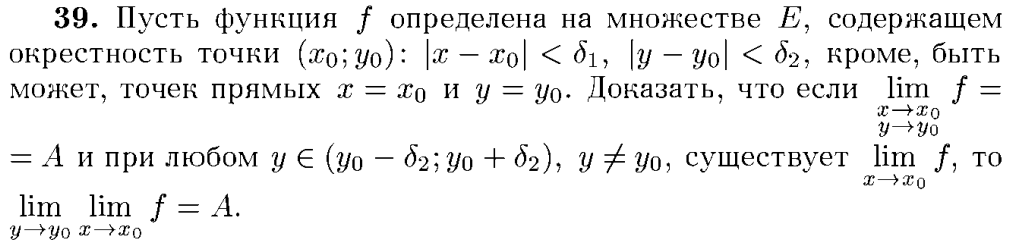
\includegraphics[scale=0.5]{./figures/239_text.png}
\end{figure}
Решение к этой задаче: \\
Рассмотрим две последовательности Гейне $x_n \to x_0$ и $y_k \to y_0$. Требуется доказать, что при условии
$$\lim_{n \to \infty} f(x_n, y_k) = B(y_k)$$ и $$\lim_{n \to \infty} f(x_n, y_n) = A$$ следует, что $$\lim_{k \to \infty} B(y_k) = A$$.
В силу существования первых двух пределов для достаточно больших $n, k$ выполняется:
$$|f(x_n, y_n) - A| < \epsilon$$
$$|f(x_n, y_k) - B(y_k)| < \epsilon$$
$$|f(x_n, y_k) - f(x_k, y_k)| < \epsilon$$
Последнее неравенство выполняется в силу фундаментальности последовательности $f(x_n, y_k)_n$.
Рассмотрим $|B(y_k) - A| \leq |B(y_k) - f(x_n, y_k)| + |f(x_n, y_k) - f(x_k, y_k)| + |f(x_k, y_k) - A| \leq 3\epsilon$. Что означает
$$\lim_{k \to \infty} B(y_k) = A$$
\section{2.4}
(а) 
$$\frac{y^2sh(x^3 - y^3)}{x^4 - x^2y^2 + y^4} = \frac{y^2(x^2 + y^2)}{x^6 + y^6} sh(x^3 - y^3)$$
Перейдя в полярные координаты и разложив $sh$ в ряд Тейлора до 1 члена в точке $(0, 0)$ получим:
$$
\rho \frac{sin^2{\phi}(cos^2{\phi} + sin^2{\phi})(cos^3{\phi} - sin^3{\phi})}{cos^6{\phi} + sin^6{\phi}} + o(\rho^4)
$$
Так как знаменатель дроби не достигает $0$, ведь одновременно $0$ синус и косинус равны быть не могут, то вся дробь ограничена и её значение меньше $K\rho$, 
где $K$ - положительная константа, тогда $K\rho$ - мажорирует выражение, а значит предел равен $0$.
\\(б)
$$f(x, y) = \frac{\arctan(x^3 + y^3)}{\sqrt{x^6 + y^6}}$$
Разложим арктангенс в ряд Тейлора и подставим в полярных координатах:
$$f(x, y) = \frac{cos^3(\phi) + \rho sin^4(\phi)}{\sqrt{cos^6(\phi) + \sin^6(\phi)}} + o(\rho)$$
Такая сумма разбивается на два слагаемых, одно из них мажорируется $\rho$, а другое от него не зависит, а значит оно зависит от направления, из чего следует несуществование предела.

\section{3.1}
$$f(x, y) = \frac{(1 - \cos(x+y) + \sin(x^2 - y^2)\ln(x^2 + y^2))}{\sqrt[3]{x^4 + x^2y^2 + y^4}}$$
Рассмотрим отдельно знаменатель дроби, переёдём к полярным координатам:
$$\frac{1}{\sqrt[3]{x^4 + x^2y^2 + y^4}} = 
\rho^{-\frac{4}{3}}\frac{1}{\sqrt[3]{\cos^4{\phi} + \sin^2{\phi}\cos^2{\phi} + \sin^4{\phi}}} = 
\rho^{-\frac{4}{3}}\frac{1}{\sqrt[3]{1 - \frac{\sin^2{2\phi}}{4}}} < 2\rho^{-\frac{4}{3}}$$
Рассмотрим числитель:
$$Q = (1 - \cos(x+y) + \sin(x^2 - y^2))\ln(x^2 + y^2) = 
(2\sin^2\left(\frac{x+y}{2}\right) + \sin(x^2 - y^2))\ln(x^2 + y^2)
$$
Тогда модуль числителя $|Q|$ меньше:
$$
|Q| \leq \left(\frac{(x+y)^2}{2} + |x^2 - y^2|\right)\ln(x^2 + y^2)
$$
Переходя к полярным координатам получим:
$$
|Q| \leq \rho^2\left(\frac{1 + \sin{2\phi}}{2} + |\cos{2\phi}|\right)\ln{\rho^2}
$$
Тогда для всей функции справедлива оценка:
$$
|f(x, y)| \leq 4\rho^{\frac{2}{3}}\ln{\rho^2} \to 0 \Rightarrow f(x, y) \to 0
$$

\section{3.2}
Перейдём к полярным координатам с учётом \(x \to  x_0\), \(y \to  y_0\) и \(y_0 = x_0\). Тогда
\[
    f(x, y) = \frac{\arctan(x_0 + \rho \cos{\phi}) - \arctan(x_0 + \rho \sin{\phi})}{\rho \cos{\phi} - \rho \sin{\phi}}
\]  
Раскладывая в ряд Маклорена относительно $\rho \to 0$:
\[
    f(x, y) = 
    \frac{x_0 + \rho \frac{1}{1 + x_0^2}\cos{\phi} + o(\rho \cos{\phi}) - x_0 - \rho \frac{1}{1 + x_0^2}\sin{\phi} - o(\rho \sin{\phi})}{\rho \cos{\phi} - \rho \sin{\phi}} = 
    \frac{1}{1 + {x_0}^{2}} + o(1)
\]
Из чего следует: 
\[
    \lim_{x, y \to x_0, x_0}{f(x, y)} = \frac{1}{1 + {x_0}^{2}} 
\]
\section{3.3}
(а) Предельная точка $x_0$ - точка для которой сущствует последовательность $x_n \to x_0$.
Тогда выберем точку $a_0 \in A^{(n + 1)}$, для неё найдём последовательность $(a_m) \to a_0 \mid a_m \in A^{(n)}$, причём для каждой из точек $a_m$
существует последовательность $(\alpha_k)_m \to a_m \mid \alpha_k \in A^{(n-1)}$. Тогда предложим последовательность $b_m = (\alpha_m)_m$. Докажем, что 
такая последовательность стремится к $x_0$. Для достаточно больших $m$:
$$
|b_m - x_0| \leq |b_m - a_m| + |a_m - x_0| \leq 2\epsilon
$$
Тогда получили, что точка $x_0$ - предельная точка $A^{(n-1)}$, то есть $x_0 \in A^{(n)} \Rightarrow A^{(n + 1)} \subset A^{(n)}$
\\(б) Рассмотрим множество $\{\frac{1}{n} \mid n \in \mathbb{N}\}$, множество её предельных точек $A^{(1)} = \{0\}$, В таком случае 
$A^{(2)} = \emptyset$, очевидно что $A^{(2)} \not = A^{(1)}$.
\\(в) Рассмотрим множество $A_n = \{0\} \cup \{\frac{1}{k_1} + ... + \frac{1}{k_n} \mid (k_1, ..., k_n) \in \mathbb{N}^n\}$. 
Очевидно, что множество $A_{n - 1} \subset A^{(1)}$, так как если $a_0 \in A_{n-1}$, то можно построить последовательность $a_n = a_0 + \frac{1}{k} \in A_n$.
Докажем, что других предельных точек нет. От противного, пусть $\exists a \in A^{(1)}, a \not \in A_{n - 1}$. Тогда существует последовательность 
$(a_n) \subset A_n \mid a_n \to a$:
$$
|\frac{1}{{k_1}_m} + ... + \frac{1}{{k_n}_m} - a| < \epsilon
$$
Выделим все стационарные подсуммы ${k_i}_m$, тогда все остальные подсуммы стремяться к $0$, а значит $a_n \to \sum_{i}{{k_i}} \in A_{n-1}$ - противоречие.
Тогда выходит, что в $(a_n)$ нет стационарных подсумм, но тогда все подсуммы стремяться к $0$, а значит $a_n \to 0 \in A_{n-1}$ - противоречие.
Тогда $A_{n-1} = A^{(1)}$ и по индукции $A_{n-k} = A^{(k)}$, соответственно $A^{(n)} = A_{0} = \{0\}$, а
$A^{(n + 1)} = A_{-1} = \emptyset$, тогда $A^{(n + 1)} \not = A^{(n)}$.
\end{document}